\documentclass[11pt, letterpaper]{article}
\usepackage[utf8]{inputenc}
\usepackage{amsmath, amssymb, amsthm}
\usepackage{geometry}
\geometry{margin=0.75in}
\usepackage{graphicx}
\usepackage{float}
\usepackage{caption}
\usepackage{siunitx}
\usepackage{booktabs}
\title{Programming Assignment 2}
\author{by Paz Lieghton}
\date{\small Applied Probability and Statistics -- Prof. Lucas Finazzi}
\begin{document}
	
	\maketitle
	
	\section*{Introduction}
	We study throughout this report the inter-arrival times of events recorded by a particle detector. This report investigates the maximum likelihood estimator (MLE) for two models: first an exponential distribution with an unknown rate of \(\lambda\), then a Gamma distribution with shape \(\alpha\) and rate \(\beta\). 
	
	The goal is to estimate parameters and assess precision, and verify the asymptotic normality of the MLE through simulations of many successions. Part~A and~B treat the exponential case (with an exponential distribution), while Part~C and~D extend to the two-parameter Gamma distribution, parameter correlation and confidence ellipses are analyzed.
	
	All simulations were performed in Python using the Spyder IDE, using the libraries: (NumPy, SciPy, Matplotlib). Random samples were drawn using a fixed seed.
	
	\section{Exponential Model: MLE and Fisher Information}
	\subsection{Log-likelihood and MLE}
	For a ample \(t_1,\dots,t_n\) from \(\text{Exp}(\lambda)\) distribution, the log-likelihood is:
	\[
	\ell(\lambda)=n\ln\lambda-\lambda\sum_{i=1}^n t_i
	\] 
	We generated \(n=200\) samples with a rate of \(\lambda_0=2.5\). The MLE satisfies \(\partial\ell/\partial\lambda=0\), yielding the form:  \(\hat{\lambda}=1/\bar{t}\). Numerically, in the python code, we obtained \(\hat{\lambda}=2.651469\) (The true value is  \(\lambda_0=2.5\)), a difference of \(0.151469\). Figure~1 shows \(\ell(\lambda)\) over a range of \(\lambda\); the maximum coincides with \(\hat{\lambda}\).
	
	\begin{figure}[H]
		\centering
		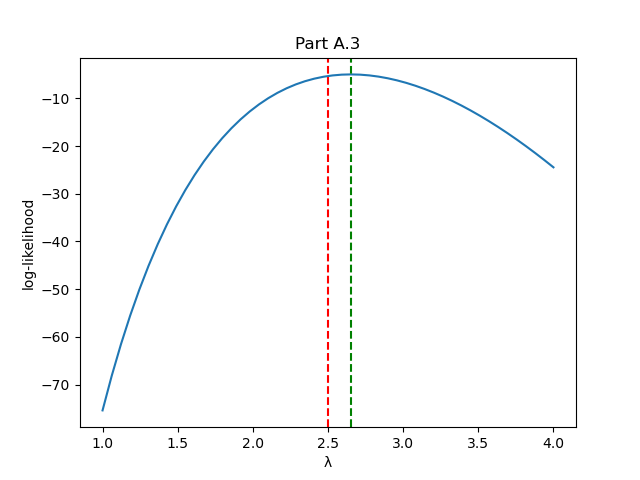
\includegraphics[width=0.65\textwidth]{fig_a3.png}
		\caption{Log-likelihood \(\ell(\lambda)\) for exponential data. Dashed red line: true \(\lambda_0=2.5\); dashed green line: MLE \(\hat{\lambda}\).}
	\end{figure}
	
	\subsection{Fisher Information and Precision}
	The Fisher information for one observation is
	\[
	I_1(\lambda)=\frac{1}{\lambda^2},
	\]
	for \(n\) observations \(I(\lambda)=n/\lambda^2\). The Cramér-Rao bound (CRB) is \(\text{Var}(\hat{\lambda})\ge \lambda^2/n\). We estimated the observed Fisher information numerically using the finite-difference approximation. (Extracted from assignment)
	\[
	\hat{I}=-\frac{\ell(\hat{\lambda}+h)-2\ell(\hat{\lambda})+\ell(\hat{\lambda}-h)}{h^2},\quad h=10^{-5}.
	\]
	The numeric value \(\hat{I}=28.45\) matched the analytic value \(n/\hat{\lambda}^2=28.45\), with a relative error of \(1.35\times10^{-5}\).
	
	To empirically assess the variance, we repeated the experiment \(M=2000\) times, each time drawing \(n=200\) samples and computing \(\hat{\lambda}_m = \frac{1}{\bar{t}_m}\). The sample variance of the 2000 estimates was \(0.0312\), while the CRB \(\lambda_0^2/n = 0.03125\) – the two are nearly identical, confirming that the MLE reaches the bound in an asymptotical way. Figure~2 displays the histogram of the 2000 estimates overlaid with the theoretical normal density \(\mathcal{N}(\lambda_0, \lambda_0^2/n)\). 
	
	The histogram fits very well with the normal curve; Poisson error bars (based on bin counts) lie within the expected fluctuations.

	\begin{figure}[H]
		\centering
		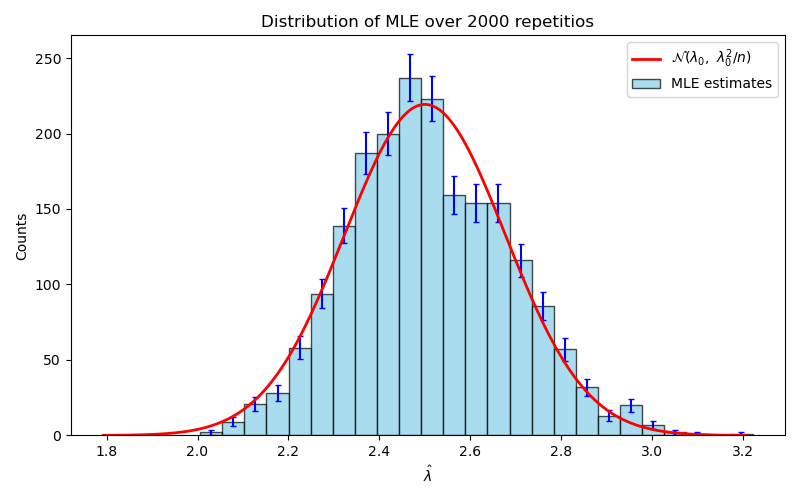
\includegraphics[width=0.7\textwidth]{fig_b5.png}
		\caption{Histogram of \(\hat{\lambda}\) from \(M=2000\) repetitions. Red curve: theoretical normal density scaled to histogram area.}
	\end{figure}
	\section{Gamma Model: Two-Parameter MLE and Covariance Matrix}
	\subsection{Data and Log-likelihood}
	We generated \(n=150\) samples from \(\text{Gamma}(\alpha_0=3,\;\beta_0=1.5)\).  
	The log-likelihood function for the Gamma distribution is
	\[
	\ell(\alpha,\beta)=n\bigl(\alpha\ln\beta-\ln\Gamma(\alpha)\bigr)+(\alpha-1)\sum_{i=1}^n\ln t_i-\beta\sum_{i=1}^n t_i .
	\]
	Because no closed‑form solution exists for \(\hat{\alpha}\), we maximized \(\ell\) numerically.  

	Starting values were extracted from the assignment PDF:
	\[
	\hat{\alpha}_{\text{start}}=\frac{\bar{t}^{\,2}}{s^{2}},\qquad 
	\hat{\beta}_{\text{start}}=\frac{\bar{t}}{s^{2}},
	\]
	where \(\bar{t}\) is the sample mean and \(s^{2}\) the sample variance. Using SciPy's minimize optimizer we found:
	\[
	\hat{\alpha}=2.5717,\qquad \hat{\beta}=1.2252,
	\]
not very close to the true parameters \(({\alpha}=3,\,{\beta}=1.5)\).
	
	\subsection{Observed Fisher Information and Correlation}
	To understand how precise our estimates are, we needed something called the observed Fisher information matrix. It's the negative of the matrix of second derivatives (the Hessian) of the log‑likelihood, evaluated at the MLE. We approximated those derivatives with small finite differences:

	\[
	\mathbf{H}=\begin{pmatrix}
		\frac{\partial^2\ell}{\partial\alpha^2} & 	\frac{\partial^2\ell}{\partial\alpha\partial\beta}\\[4pt]
		\frac{\partial^2\ell}{\partial\alpha\partial\beta} & \frac{\partial^2\ell}{\partial\beta^2}
	\end{pmatrix}_{\!(\hat{\alpha},\hat{\beta})}.
	\]

	The covariance matrix of \(\hat{\alpha}\) and \(\hat{\beta}\) is then \((-\mathbf{H})^{-1}\). The numbers we got in the program were:

	\[
	\hat{\boldsymbol{\Sigma}}=\begin{pmatrix}
		0.078310 & 0.037309\\
		0.037309 & 0.021667
	\end{pmatrix}.
	\]

	From that, the correlation between \(\hat{\alpha}\) and \(\hat{\beta}\) is about \(0.9058\), a very strong correlation. The gamma mean is \(\alpha/\beta\), so if the data pushes the mean estimate up, both parameters tend to increase together. 
	
	\section{The Multivariate Normal and Confidence Ellipses}
	\subsection{Repeated Sampling and Covariance Comparison}
	We repeated the full Gamma estimation \(M=2000\) times, storing each pair \((\hat{\alpha}_m,\hat{\beta}_m)\). The sample covariance matrix of these values was:
	
	\[
	\mathbf{S}=\begin{pmatrix}
		0.111373 & 0.056737\\
		0.056737 & 0.034351
	\end{pmatrix},
	\]
	which is slightly bigger than the theoretical \(\hat{\boldsymbol{\Sigma}}\) from the Hessian we calculated on the previous section.
	
	\subsection{Ellipses and Coverage}
	A bivariate normal distribution:
	\[
	d^2(\boldsymbol{\theta})=(\boldsymbol{\theta}-\boldsymbol{\theta}_0)^\top\hat{\boldsymbol{\Sigma}}^{-1}(\boldsymbol{\theta}-\boldsymbol{\theta}_0)
	\]
	Follows a \(\chi^2\) distribution with 2 degrees of freedom. Confidence ellipses at levels \(68\%\), \(90\%\), and \(95\%\) were constructed. Figure~3 shows the scatter plot of the 2000 MLE pairs together with the three ellipses centred at the MLE from the original single run. The ellipses tilt positively, reflecting the strong correlation between \(\hat{\alpha}\) and \(\hat{\beta}\).
	
	\begin{figure}[H]
		\centering
		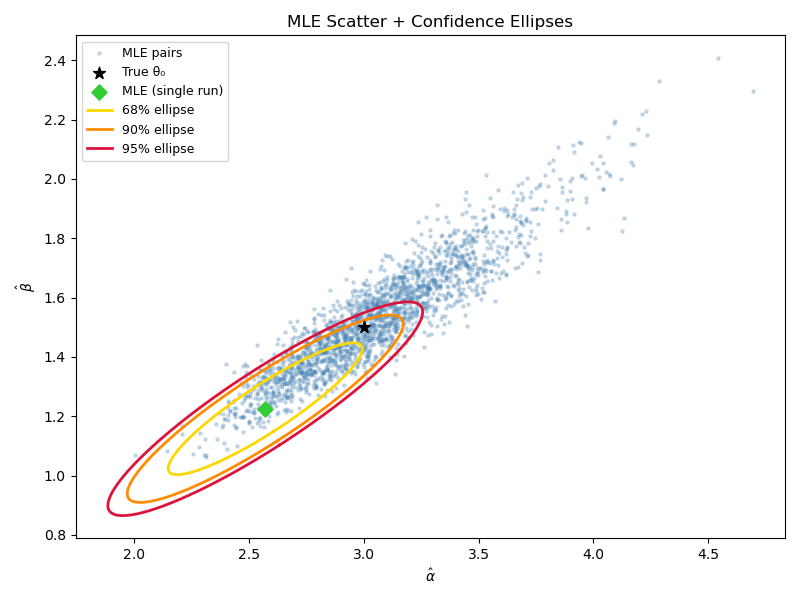
\includegraphics[width=0.75\textwidth]{fig_d3.png}
		\caption{Scatter plot of 2000 \((\hat{\alpha},\hat{\beta})\) pairs. Black star: true parameters; green diamond: MLE from single run; ellipses: 68\%, 90\%, 95\% confidence regions.}
	\end{figure}

	\[
	\begin{array}{ccc}
		\text{Nominal level} & \chi^2_{2,p} & \text{Empirical coverage}\\\hline
		68\% & 2.28 & 0.2580\\
		90\% & 4.61 & 0.4695\\
		95\% & 5.99 & 0.5610
	\end{array}
	\]
	The empirical coverages are notably lower than the nominal levels. I suppose due to the lack of tests done, n = 150.
	In my code if I change that value, the scatter plot approximates the confidence elipses with way more precision and 	the empirical coverage raises dramatically., so the issue is that very value.

	
	\subsection{Marginal Histograms}
	Figure~4 presents histograms of \(\hat{\alpha}\) and \(\hat{\beta}\) separately, with Poisson error bars and the theoretical normal curves \(\mathcal{N}(\alpha_0,\hat{\Sigma}_{11})\) and \(\mathcal{N}(\beta_0,\hat{\Sigma}_{22})\). Both histograms are reasonably similar to the normal densities
	
	\begin{figure}[H]
		\centering
		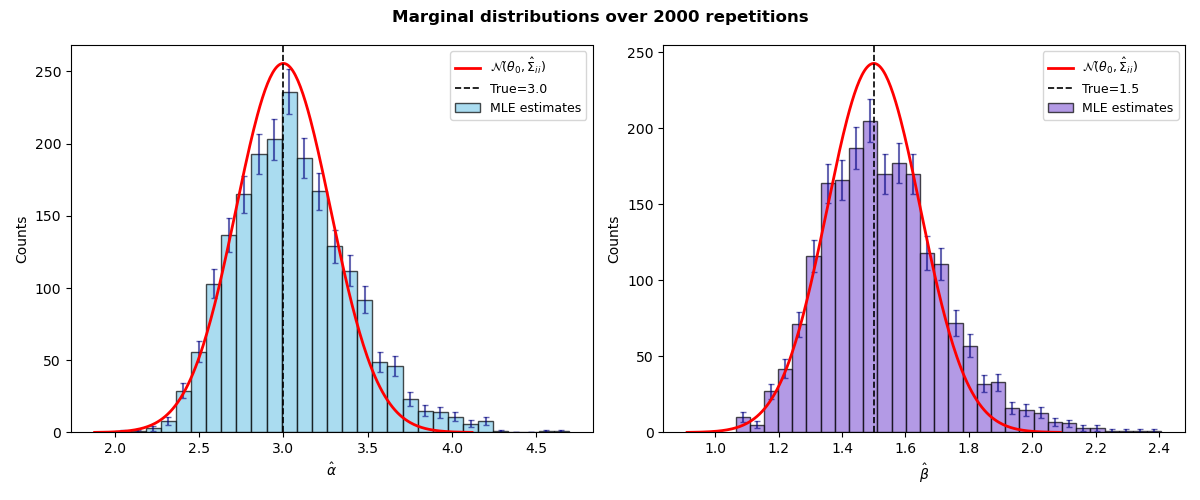
\includegraphics[width=0.9\textwidth]{fig_d6.png}
		\caption{Marginal distributions: left \(\hat{\alpha}\), right \(\hat{\beta}\). Red dashed curve: theoretical normal based on \(\hat{\boldsymbol{\Sigma}}\). Black vertical lines are the true parameter values.}
	\end{figure}
	
\section*{Conclusion}
We fitted an exponential model to 200 observations and a Gamma model to 150 observations. In the exponential case the MLE formula is known, and our simulation showed that the variance of the estimator matched the Cramér‑Rao bound, as expected. 

In the Gamma case we had to use numerical optimization to find the shape and rate. The estimated parameters turned out strongly correlated, which makes sense because the mean of a Gamma is \(\alpha/\beta\).We repeated the estimation many times, the spread of the pairs was larger than the theoretical covariance matrix predicted, and the confidence ellipses captured fewer points than the nominal levels said they should. Because of the value of n.
Still, the histograms of \(\hat{\alpha}\) and \(\hat{\beta}\) closely approximate a normal density.
\section*{Sources}
\begin{itemize}
	\item Python Graph Gallery. Matplotlib examples and reference. \texttt{https://python-graph-gallery.com}
	\item Cowan, Glen. \textit{Statistical Data Analysis}. Oxford University Press, 1998.
	\item AI Assistance: DeepSeek was used for the Gamma model and specially plotting of Figures 3 and specially the 4th one.
\end{itemize}
\end{document}